\documentclass[11pt,reqno,final]{amsart}

\pdfcompresslevel=0
\pdfobjcompresslevel=0

\usepackage[dvipsnames]{xcolor}% adds colors
\usepackage{amsmath, amsthm}% {amsfonts, amssymb}

% New Characters

\usepackage[latin1]{inputenc}%
\usepackage[T1]{fontenc}
\usepackage{MnSymbol}
\usepackage[theoremfont,largesc]{newpxtext}
\usepackage{newpxmath}

\usepackage[normalem]{ulem}% underlining
\usepackage{bbm}% more bb
%\usepackage{dsfont}% double strike-through
% \usepackage{upgreek}

\usepackage[inline,shortlabels]{enumitem}% % can use \begin{enumerate*} for inparaenum


% Page Typesetting
\usepackage[final]{microtype}
\usepackage{relsize}
\usepackage[margin=1in]{geometry}
\usepackage{framed}
\usepackage{pdfpages}

\usepackage{hyperref}
\hypersetup{
  final,
  pdftitle={Math 135 09-04_Bottles},
  % pdfauthor={Bonventre}, 
  linktoc=page,
  pagebackref,
  colorlinks=true,
  citecolor=PineGreen,
  linkcolor=PineGreen,
  linkbordercolor=PineGreen,
}

% Internal references

\numberwithin{equation}{section} 
\numberwithin{figure}{section}

\usepackage[nameinlink,capitalise,noabbrev]{cleveref}
\crefname{equation}{}{} % get \cref to behave as \eqref

% \theoremstyle{plain} % bold name, italic text
\newtheorem{theorem}[equation]{Theorem}%
\newtheorem*{theorem*}{Theorem}%
\newtheorem{claim}[equation]{Claim}%
\newtheorem{question}{Question}

\theoremstyle{definition} % bold name, plain text
\newtheorem{definition}[equation]{Definition}%
\newtheorem*{definition*}{Definition}%
\newtheorem{example}[equation]{Example}%
\newtheorem*{example*}{Example}%
\newtheorem{remark}[equation]{Remark}%
\newtheorem{exercise}[question]{Exercise}

% macros

\newcommand{\set}[1]{\left\{#1\right\}}%
\newcommand{\sets}[2]{\left\{ #1 \;|\; #2\right\}}%
\newcommand{\longto}{\longrightarrow}%
\newcommand{\into}{\hookrightarrow}%
\newcommand{\onto}{\twoheadrightarrow}%

\usepackage{harpoon}
\newcommand{\vect}[1]{\text{\overrightharp{\ensuremath{#1}}}}

\newcommand{\del}{\partial}%

\newcommand{\ki}{\chi}
\newcommand{\ksi}{\xi}
\newcommand{\Ksi}{\Xi}


% %%%%%%%%%%%%%%%%%%%%%%%%%%%%%%%%%%%%%%%%%%%%%%%%%%%%%%%%%%%%%%%%%%%%%%%%%%%%%%%%%%%%%%%%%%%%%%%%%%%%
% Document body

\begin{document}

\begin{center}
        \textbf{\Large Math 135, Calculus 1, Fall 2020}\\[10pt]
        {\large 09-04: Functions (Section 1.1)}
\end{center}

\thispagestyle{empty}

% \vspace{-1em}


\renewcommand{\thesection}{\Alph{section}}
\section{Meet your Classmates}

Share and discuss with your classmates your ``\sout{Desert Island} Quarantine 5'':
\begin{question}
        If you were to be isolated on a desert island/apartment/your parent's house (say with an infinite supply of food and water), what 5 items would you want to have with you?
\end{question}
\vfill

\section{Filling Bottles}
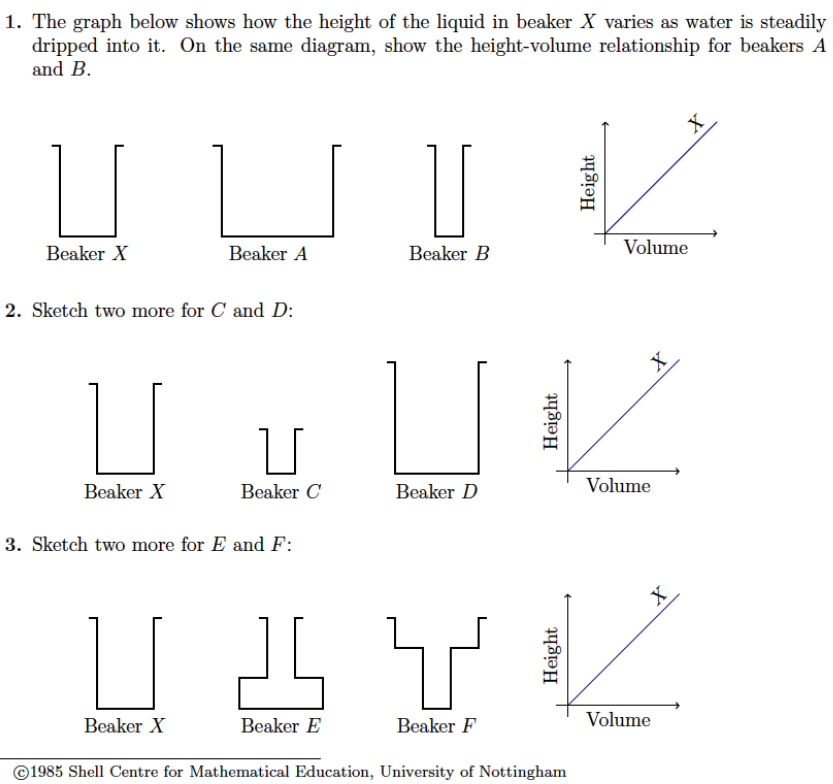
\includegraphics[width=\textwidth]{09-04P_FillingBottles1}

\newpage
\newgeometry{margin=1in}

\begin{exercise} \textbf{Explain your reasoning}

\begin{enumerate}[label=(\alph*), leftmargin=*]
\item Do the diagrams on the previous page describe functions?  Justify your answer by providing a definition of function.
        \vfill
\item What is the independent variable in each of the diagrams above?  What is the dependent variable?
        \vfill
\item How do the domain and range of the relation described by Beaker A compare with the domain and range of the relation described by Beaker X?  How is this reflected in the shape of the graph?
        \vfill
        How do the domain and range of the relation described by Beaker B compare with the domain and range of the relation described by Beaker X?  
        \vfill
\item How do the domain and range of the relation described by Beaker C compare with the domain and range of the relation described by Beaker X?  How is this reflected in the shape of the graph?
        \vfill
        How do the domain and range of the relation described by Beaker D compare with the domain and range of the relation described by Beaker X?  How is this reflected in the shape of the graph?
        \vfill
\item How do the domain and range of the relation described by Beaker E compare with the domain and range of the relation described by Beaker X?  How is this reflected in the shape of the graph?
        \vfill
        How do the domain and range of the relation described by Beaker F compare with the domain and range of the relation described by Beaker X?  How is this reflected in the shape of the graph?
        \vfill
\end{enumerate}
\end{exercise}
\newpage

\section{Properties of Functions}

\begin{framed}
        We say that a function $f$ is {\bf increasing} on an interval $I$ if 
        \[
                f(x_1) \; < \; f(x_2) \quad \mbox{whenever }  x_1 < x_2  \mbox{ in } I.
        \]
        Likewise, 
        $f$ is {\bf decreasing} on an interval $I$ if 
        \[
                f(x_1) \; > \; f(x_2) \quad \mbox{whenever } x_1 < x_2 \mbox{ in } I.
        \]
\end{framed}

\begin{exercise}
        All of the functions we have seen above are increasing.  Given the context, why is this the case?  What would it mean for a function to be decreasing?
        \vfill
\end{exercise}

\begin{exercise}
        Is it possible to create a function $f(x)$ with the following properties?  If so, create it.  If not, explain why not.
        \begin{itemize}
        \item The domain of $f(x)$ is $[-4,4]$.
        \item The range of $f(x)$ is $[-20,10]$.
        \item $f(-4)=-6$
        \item $f(-2)=8$
        \item $f(1)=-16$
        \item $f(x)$ is increasing on the intervals $[-4,-2)$ and $(1,4]$
        \item $f(x)$ is decreasing on the interval $(-2,1)$
        \end{itemize}
        \vfill
        \vfill
\end{exercise}

\newpage

\begin{framed}
        We say a function is \textbf{even} if $f(-x) = f(x)$ for all $x$ in its domain.
        The graph of an even function is symmetric about the vertical axis.  
        
        Likewise, we say a function is \textbf{odd} if $f(-x) = -f(x)$ for all $x$ in its domain.
        The graph of an odd function is symmetric ``about the origin''
        (the graph is the same after rotating about the origin by 180 degrees).
\end{framed}

\begin{exercise}
        Below, sketch the graph of an even function, an odd function, and a function that is neither even nor odd.
        \vfill
\end{exercise}

\begin{exercise}
        Is it possible to create a function $f(x)$ with the following properties?  If so, create it.  If not, explain why not.
        \begin{itemize}
        \item $f(x)$ is even.
        \item The domain of $f(x)$ is $[-4,4]$.
        \item The range of $f(x)$ is $[-20,10]$.
        \item $f(-4)=-6$
        \item $f(-2)=8$
        \item $f(1)=-16$
        \item $f(x)$ is increasing on the intervals $[-4,-2)$ and $(1,4]$
        \item $f(x)$ is decreasing on the interval $(-2,1)$
        \end{itemize}
        \vfill
\end{exercise}

\newpage

\begin{framed}
        The piecewise definition for $|x|$ is
        \[
                |x| =
                \begin{cases}
                        x \qquad & \mbox{if $x \geq 0$}\\
                        -x & \mbox{if $x < 0$}
                \end{cases}
        \]
        Written this way, we see that $|x|$ is an example of a \textbf{piecewise function}.
\end{framed}
We'll use this definition a lot throughout the course.  For example, it's useful for solving inequalities.

$ $

\begin{exercise}
        Describe your answers using interval notation and draw them on the number line.
        \begin{enumerate}[(a)]
        \item Where is $|2x-3|\leq 4$? \\
                \vspace{30pt}\\
        \item Where is $|2x-3|>4$?\\
                \vspace{30pt}\\
        \item What is the relationship between the answers you found in (1) and (2)?
        \end{enumerate}
\end{exercise}


\newpage

\section{Bonus Bottle Problems}

$ $

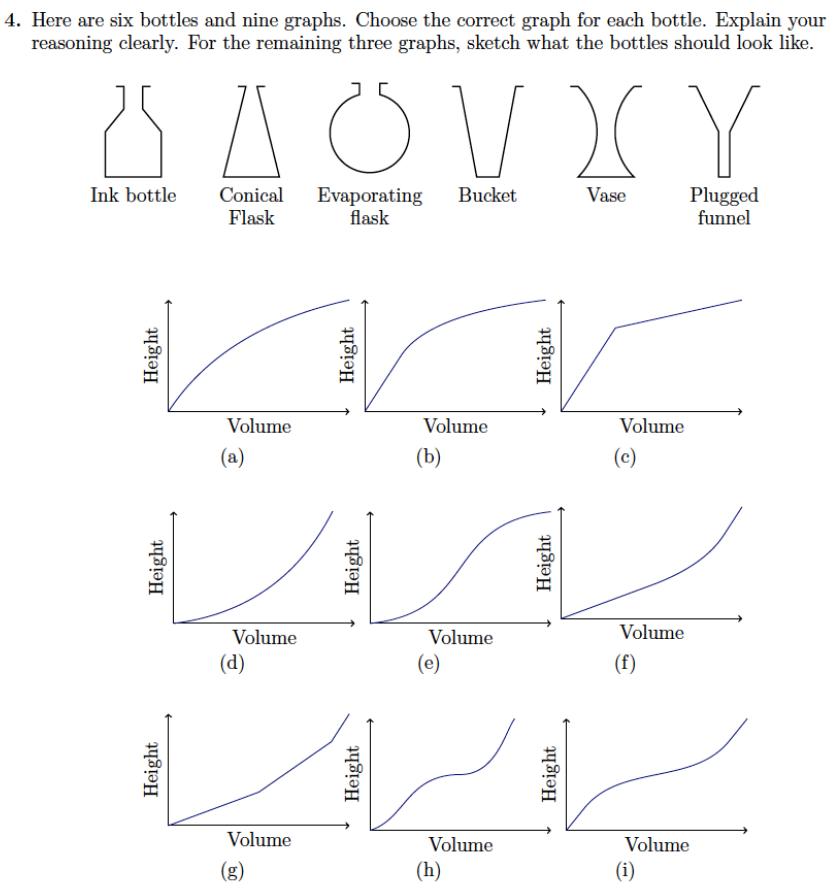
\includegraphics[width=\textwidth]{09-04P_FillingBottles2.png}

\newpage


\end{document}